\documentclass[12pt]{extarticle}
\usepackage[margin=1in]{geometry}
\usepackage{amssymb}
\usepackage{amsmath}
\usepackage{url}
\usepackage{bm}
\usepackage{color}
\usepackage{graphicx}

\title{Notes on Siemens Elements of Nuclei}
\author{Cody L. Petrie}

\begin{document}
\maketitle

\section*{Chapter 3}
\subsection*{The Black Sphere}
To talk about the scattering of a neutron from some nuclei we are first going to consider scattering from an absorbing spherical object. We start by assuming the incident neutron beam is a plane wave $e^{ikz}$. We then expand this plane wave in terms of legendre polynomials in the scattering regiem.

Expanding a plane wave in the spherical harmonic basis gives
\begin{equation}
   e^{i\mathbf{k}\cdot\mathbf{r}} = \sum\limits_l C_l Y_l^0(\theta).
\end{equation}
There is no $\phi$ dependance here because the plane wave only depend on $\theta$ the angle between $\mathbf{k}$ and $\mathbf{r}$, since the plane wave is propagating in the z direction. Now solving for the expansion coefficients $C_l$ using the orthogonality relationship
\begin{equation}
   \int_0^{\pi} \int_0^{2\pi} Y_l^m Y_{l'}^{m'*} d\Omega = \delta_{ll'}\delta_{mm'},
\end{equation}
gives us
\begin{equation}
   C_l = 2\pi \int_0^{\pi} e^{ikr\cos\theta}Y_l^0(\theta)\sin\theta d\theta.
\end{equation}
Now writting the spherical harmonics in terms of legendre polynomials
\begin{equation}
   Y_l^m(\theta,\phi) = \sqrt{\frac{2l+1(l-m)!}{4\pi(l+m!)}}P_l^m(\cos\theta)e^{im\phi},
\end{equation}
or for $m=0$,
\begin{equation}
   Y_l^0(\theta)=\sqrt{\frac{2l+1}{4\pi}}P_l(\cos\theta)
\end{equation}
we get,
\begin{equation}
   C_l = \pi \int_0^\pi e^{ikr\cos\theta}\sqrt{\frac{2l+1}{4\pi}}P_l(\cos\theta) \sin\theta d\theta.
\end{equation}
Now if you use an identity relating the spherical bessel functions of the first kind to the legendre polynomials (an identity which I found online and proved with Mathematica)
\begin{equation}
   j_l(kr)=\frac{1}{2i^l}\int_0^\pi e^{ikr\cos\theta}P_l{\cos\theta},
\end{equation}
we can get an expansion of the plane wave in terms of spherical bessel functions and legendre polynomials.
\begin{equation}
   \boxed{e^{ikz} = \sum\limits_l 2i^l \sqrt{\pi}\sqrt{2l+1} j_l(kr)Y_l^0(\theta)}
\end{equation}
Often we want to look at these things in the scattering or radiation limit where r is large. We can use the expansion of the spherical bessel function as given by Jackson eq. 9.89 to be
\begin{equation}
   \lim\limits_{r->\infty} j_l(kr) = \frac{1}{kr} \sin\left( kr-\frac{l\pi}{2} \right) = \frac{i}{2kr}(e^{-i(kr-\frac{l\pi}{2}) - e^{i(kr-\frac{l\pi}{2})}}).
\end{equation}
We can thus write the expansion in the asymptotic limit as
\begin{equation}
   \boxed{e^{ikz} \approx \sum\limits_l \frac{\sqrt{\pi}}{kr} \sqrt{2l+1} \, i^{l+1} \left( e^{-i(kr-\frac{l\pi}{2})} - e^{i(kr-\frac{l\pi}{2})} \right) Y_l^0(\theta)}.
\end{equation}
This is equation 3.1.1 in Siemens.


The scattering is going to happen for some finite amount of time while the nucleon interacts with the nucleus and then the scattering interaction will turn off. After the interaction has turned off we can imaging that the amplitude of outgoing wave, $e^{i(kr-\frac{l\pi}{2})}$ has been modified giving us a wave function of
\begin{equation}
   \phi(r\rightarrow\infty) = \sum\limits_l \frac{\sqrt{\pi}}{kr} \sqrt{2l+1} \, i^{l+1} \left( e^{-i(kr-\frac{l\pi}{2})} - \eta_l e^{i(kr-\frac{l\pi}{2})} \right) Y_l^0(\theta).
\end{equation}
Now we can get the scattered wave $\phi_s$ by subtracting the incident plane wave from this since $\phi = \phi_i + \phi_s$.
\begin{align}
   \phi_s &= \sum\limits_l \frac{\sqrt{\pi}}{kr} \sqrt{2l+1} \, i^{l+1} \left( e^{-i(kr-\frac{l\pi}{2})} - \eta_l e^{i(kr-\frac{l\pi}{2})} - e^{-i(kr-\frac{l\pi}{2})} + e^{i(kr-\frac{l\pi}{2})} \right) Y_l^0(\theta) \\
   &= \sum\limits_l \frac{\sqrt{\pi}}{kr} \sqrt{2l+1} \, i^{l+1} e^{i(kr-\frac{l\pi}{2})}(1 - \eta_l) Y_l^0(\theta) \\
   &= \sum\limits_l i \frac{\sqrt{\pi}}{kr} \sqrt{2l+1} e^{ikr}(1 - \eta_l) Y_l^0(\theta) \\
   &= f(\theta) \frac{e^{ikr}}{r}
\end{align}
Where in the last line I have used the face that $i=e^{\pi/2}$, and where
\begin{equation}
   f(\theta) = \sum\limits_l i \frac{\sqrt{\pi}}{k}\sqrt{2l+1} Y_l^0(\theta) (1-\eta_l)
\end{equation}

Putting these together we get
\begin{equation}
   \phi(r\rightarrow\infty) = e^{ikz} + f(\theta)\frac{e^{ikr}}{r},
\end{equation}
where we can recognize the $f(\theta)$ term as being part of the differential scattering cross section, $\frac{d\sigma}{d\Omega} = \left|f(\theta)\right|^2$.

Now let's make some approximations. Siemens says that the classical turning point for a neutron is when $k^2 = l(l+1)/R^2 \approx (l+\frac{1}{2})^2/R^2$. Solving this for l gives $l=kR-\frac{1}{2}$. Now, if a particle passes within the range $R$ then we can say that it is absorbed and $\eta_l=0$. This happens for small angular momentum $l < kR-\frac{1}{2}$. But for large enough angular momentum, $l > kR - \frac{1}{2}$, the particles pass too far away to be scattered and the scattered wave is the same as the incident plane wave, $\eta_l=1$, which gives $\frac{d\sigma}{d\Omega} = 0$, thus we only need to sum to $l=kR-\frac{1}{2}$. Finally this gives us the differential scattering cross section.
\begin{equation}
   \frac{d\sigma}{d\Omega} = \frac{\pi}{k^2} \left|\sum\limits_{l=0}^{kr-1/2} \sqrt{2l+1} Y_l^0(\theta)\right|^2
\end{equation}
The next thing Siemens does is to approximate these for large and small scattering angles. I had a hard time doing the integrals they did so I'll just quote the results here. These are equations 3.1.9a and 3.1.9b in the book.
\begin{align}
   \frac{d\sigma}{d\Omega} \approx
\begin{cases}
   \frac{2R}{\pi} k\theta^2 \sin\theta\cos^2\left(kR\theta+\frac{\pi}{4}\right),& \text{for } kR\theta \gg 1 \\
   \frac{k^2R^4}{4}(1-(kR\theta/2)^2)^2,& \text{for } kR\theta \ll 1
\end{cases}
\label{eq:crossapprox}
\end{align}
I have plotted these two as in figure 3.2 of the book. My reproduction isn't exactly like there's but it is roughly the same.
\begin{figure}[h]
   \centering
   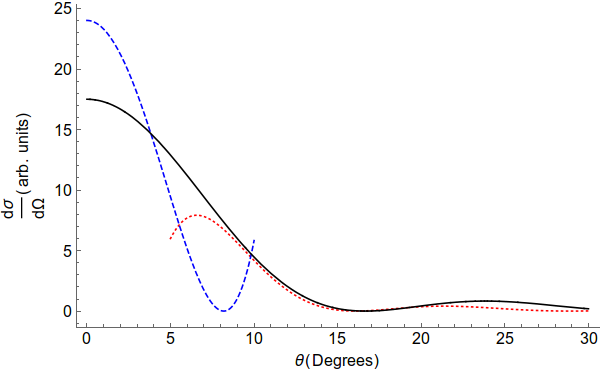
\includegraphics[width=0.5\textwidth]{fig3_2.png}
   \caption{Comparison of approximations where R=7 and k=2. The dashed curve is low angle approximate and the dotted curve is the high angle approximation.}
\end{figure}

\subsection*{Nuclear Sizes and the Saturation of Nuclear Forces}
We can use these expressions to learn about the radius of the nucleus. For example if we look for the minimum of the large angle of equation~\ref{eq:crossapprox} we get an expression in terms of the radius.
\begin{align}
   \frac{d}{d\theta}\frac{d\sigma}{d\Omega} &= -\frac{2R}{\pi k\theta^2\sin\theta}2\cos\left(kR\theta+\frac{\pi}{4}\right) + \frac{2R}{\pi k}\cos^2\left(kR\theta+\frac{\pi}{4}\right)\left(-\frac{2}{\theta^3\sin\theta}-\frac{\cos\theta}{\theta^2\sin^2\theta}\right) \\
   &= -\frac{4R}{\pi k\theta^2\sin\theta}\cos\left(kR\theta+\frac{\pi}{4}\right) \left[1 + \cos\left(kR\theta+\frac{\pi}{4}\right)\left(-\frac{1}{\theta}-\frac{1}{2}\frac{\cos\theta}{\sin\theta}\right)\right] \\
\end{align}
This is zero when the argument of the $\cos$ is $n\frac{\pi}{2}$, where n is some integer. So solving $kR\theta+\frac{\pi}{4} = n\frac{\pi}{2}$ we get
\begin{equation}
   \theta_{min} = \frac{\pi}{4kR}(2n-1).
\end{equation}
For some reason (I assume based on where the first minimum in the experimental curves is located) Siemens says that
\begin{equation}
   \boxed{ \theta_{min} = \frac{5\pi}{4kR} }.
\end{equation}
Or equivalently for the nuclear volue $\Omega_r$.
\begin{equation}
   \Omega_r = \frac{4}{3}\pi R^3 = \frac{125}{48}\frac{\pi^4}{(k\theta_{min})^3}
\end{equation}
He then goes to say based on figure 3.1 in his book that if $\epsilon = 84$ MeV for Pb, where $k = \sqrt{2m_n\epsilon/\hbar^2} \approx 2.0$ fm$^{-1}$, and with $\theta_{min} \approx 15^\circ$ you get an esimated radius of lead to be $7.5$ fm. A quick google search shows that the radius is somewhere around $7$ fm.

\end{document}
